\chapter{Background and Related Work}

\section{Common Terminology}
Before detailing the background relating to ASP \cite{Lifschitz1999}, a list of common terms that will be used throughout can be found in Table \ref{table:4}.

\begin{table}[p!]
\centering
\makeatletter
\@fpsep\textheight
\makeatother
\begin{tabular}{| c | m{0.7\linewidth} |}
\hline
Constant & 
\mbox{}\newline
A sequence of characters starting with a lower case character or number. Typically denoted \lstinline!a, b, c, ... p, q, r, ...!. \newline
\\
\hline
Variable & 
\mbox{}\newline
A character or sequence of characters starting with an upper case letter, representing some range of possible constants. Typically denoted \lstinline!A, B, C, ... X, Y, Z, ...!.\newline
\\
\hline
Term &
\mbox{}\newline
Either a constant or a variable \newline
\\
\hline
Predicate &
\mbox{}\newline
A character or sequence of characters representing some relation between Constants or Variables. For example, the predicate \lstinline!on, above, below!. \newline
 \\
\hline
Atom &
\mbox{}\newline
A predicate applied to some terms. \lstinline!on(X, Y), above(a, b), p(X), q(Z)! are all examples of atoms.\newline
 \\
\hline
Literal & 
\mbox{}\newline
Either an Atom or an Atom preceded by the \lstinline!not! operator, representing Negation By Failure. \newline
\\
\hline
Rule & 
\mbox{}\newline
A line of the form \lstinline!head :- body! where \lstinline!head! is an atom and \lstinline!body! is a list of literals.
\newline
 \\
\hline
Program &
\mbox{}\newline
A conjunction of rules \newline
\\
\hline
\end{tabular}
\caption{Common Logic Terms \cite{Muggleton1991}}
\label{table:4}
\clearpage
\end{table}

\section{Answer Set Programming}

\subsection{Negation As Failure}
Negation as failure is an inference rule used in non-monotonic logic programs to derive atoms of the form \lstinline!not p!. This derivation is defined as 
\begin{displayquote}
``\lstinline!not p! can be inferred if every possible proof of \lstinline!p! fails.'' \cite{negAsFailure}
\end{displayquote}
In more simple terms, this means that you can assume that \lstinline!not p! holds if you cannot prove \lstinline!p!. 
As an example, consider the program \\

\begin{lstlisting}
p :- not q.
q :- r.
\end{lstlisting}
\mbox{}\\
As \lstinline!q! cannot be proven, we can instead prove \lstinline!not q!, which is then used to prove \lstinline!p!.

\subsection{The Stable Model Semantics}

The Stable Model Semantics \cite{KRnotes} provides a natural semantics for both normal and extended logic programs, in which instead of giving individual solutions to queries we define a set of ``Answer Sets'' (Stable Models) of the program. For example, given the program: \\

\begin{lstlisting}
p :- not q.
q :- not p.
\end{lstlisting}
\mbox{}\\
The value of p depends on the value of q, so when you query Prolog for p? this program results in an infinite search, alternately searching for p and q until cancelled. However, using the Stable Model Semantics, this particular program has an answer set for each solution : \lstinline!{p}! and \lstinline!{q}!.

\subsubsection{Grounding}

Before you can solve a logic program using Answer Sets you must first ground it \cite{KRnotes}. A rule is said to be ``ground'' if all of its variables are replaced by every combination of possible constants. Then, to calculate the grounding of a program P you replace each rule in P by every ground instance of that rule. For example, the program \\

\begin{lstlisting}
p(1, 2).
q(X) :- p(X, Y), not q(Y).
\end{lstlisting}
\mbox{}\\
has grounding \\

\begin{lstlisting}
p(1,2).
q(1) :- p(1, 1), not q(1).
q(1) :- p(1, 2), not q(2).
q(2) :- p(2, 1), not q(1).
q(2) :- p(2, 2), not q(2).
\end{lstlisting}
\mbox{}\\
This is calculated as the grounding for this program, because the variables \lstinline{(X, Y)} in the rule \lstinline{q(X) :- p(X, Y), not q(Y).} are replaced by all possible combinations of the constants \lstinline{(1, 2)}. These combinations are, specifically :\\%{

\begin{lstlisting}
{ X = 1, Y = 1 }
{ X = 1, Y = 2 }
{ X = 2, Y = 1 }
{ X = 2, Y = 2 }
\end{lstlisting}

\subsubsection{Safety}

Because of the need for ASP solvers to ground the entire program, they are restricted to safe rules \cite{Cabalar2009}. A rule is safe if every variable in that rule occurs positively in the body of the rule. Some examples of unsafe rules are:

\begin{itemize}
\item \lstinline!p(X) :- q(Y).! Unsafe because the variable \lstinline!X! does not appear in the body. 
\item \lstinline!p(Z) :- not q(X, Y), r(X, Y).! Unsafe because the variable \lstinline!Z! does not appear the body of the rule.
\item \lstinline!p(X) :- q(X), not r(Y).! Unsafe because the variable \lstinline!Y! does not appear positively in the body.
\end{itemize}

\pagebreak

\subsubsection{Least Herbrand Models}
For a normal logic program P, the following features are defined as follows \cite{KRnotes} :

\begin{center}
\begin{tabular}{| c | m{0.7\linewidth} |}
\hline
Herbrand Base & 
\mbox{}\newline
The set of all ground atoms of a program.\newline
\\
\hline
Herbrand Interpretation & 
\mbox{}\newline
An assignment on the Herbrand Base, specifying which ground atoms are true and which are false.\newline \newline
A rule is satisfied by an interpretation if, when all atoms of the body are specified as true in the interpretation, then so is the head of the rule.\newline
\\
\hline
Herbrand Model & 
\mbox{}\newline
A Herbrand Interpretation where every rule in the program is satisfied by that interpretation.\newline \newline
A Herbrand Model M is minimal if no subset of M is also a model. For definite logic programs this model is unique and called the least Herbrand Model, however this does not always hold for normal or extended logic programs.\newline
\\
\hline
\end{tabular}
\end{center}
\mbox{}\\
For example, consider the program P:\\

\begin{lstlisting}
p :- not q.
q :- not p.
\end{lstlisting}
\mbox{}\\
P has the Herbrand Base \lstinline!{p, q}!. \\ \\ 
Because listing if each atom is true or false is overly verbose, instead we write the Herbrand Interpretation as a set of atoms, including the ones specified as true. One Herbrand Interpretation of P is \lstinline!{p, q}!, but this interpretation is not a model because neither rules are satisfied by it. \\ \\
The Herbrand Interpretations \lstinline!{p}! and \lstinline!{q}! are both Herbrand Models. \lstinline!{p}! is a model because it satisfies the both rules - the first as \lstinline!not q! holds by NBF and \lstinline!p! is in the model, and the second as \lstinline!(not p)! does not hold so \lstinline!q! is not needed. \lstinline!{q}! is a Herbrand Model for the same reasons, reversed. The first line is satisfied because the body \lstinline!not q! does not hold, and the second line is satisfied as \lstinline!not p! holds, and \lstinline!q! is in the interpretation.

\subsection{Calculating Answer Sets}

\subsubsection{Reduct}

Let P be a ground normal logic program, and X be a set of atoms. The reduct \cite{Law2015} of P, P\textsuperscript{X} is calculated from P by :

\begin{enumerate}
\item Delete any rule from P which contains the negation as failure of an atom in X.
\item Delete any negation as failure atoms from the remaining rules in P.
\end{enumerate}
We then say X is an Answer Set (Stable Model) of P if it is a least Herbrand Model of  P\textsuperscript{X}. For example, if program P is:\\

\begin{lstlisting}
p(1, 2).
q(1) :- p(1, 1), not q(1).
q(1) :- p(1, 2), not q(2).
q(2) :- p(2, 1), not q(1).
q(2) :- p(2, 2), not q(2).
\end{lstlisting}
\mbox{}\\
First, try X = \lstinline!{q(1)}!. The reduct is calculated as : \\

\begin{lstlisting}
p(1, 2).
q(1) :- p(1, 2).
q(2) :- p(2, 2).
\end{lstlisting}
\mbox{}\\
The Least Herbrand Model of this reduct is \lstinline!{p(1, 2), q(1)}!. Therefore X is not an Answer Set of P. \\ \\
Then, when trying X = \lstinline!{p(1,2), q(1)}!, the reduct is:\\

\begin{lstlisting}
p(1, 2).
q(1) :- p(1, 2).
q(2) :- p(2, 2).
\end{lstlisting}
\mbox{}\\
A Least Herbrand Model M(P\textsuperscript{X}) = \{p(1,2), q(1)\}, so X is an Answer Set of P. \\ \\
It is important to note that Answer Sets are not unique and some programs might have no Answer Sets.

\subsubsection{Constraints}

Constraints \cite{ASPnotes} are a way of filtering out unwanted Answer Sets. They are written as rules with an empty head, which is equivalent to $\bot$. Semantically, this means that any model which satisfies the body of the constraint cannot be an Answer Set. For example, the program with constraint : \\

\begin{lstlisting}
p :- not q.
q :- not p.
:- p, not q.
\end{lstlisting}
\mbox{}\\
Has only one Answer Set, \lstinline!{q}!. This is because the Answer Set \lstinline!{p}! fails the constraint, as it contains \lstinline!p! and does not contain \lstinline!q!.

\subsubsection{Aggregates and Choice Rules}

An aggregate \cite{Eiter2008} is a ASP atom with the format $a \: \textsf{op} \: [h_1=w_1, h_2=w_2, \dots, h_n=w_n 	] \: b$. An aggregate is satisfied by an interpretation X if operation op applied to the multiset of weights of true literals is between the upper and lower bounds $a$ and $b$. \\ \\
This project will be using one application of aggregates, the choice rule. A choice rule has an aggregate using the count operation as the head of the rule, and semantically represents a choice of a number of head atoms, between the upper and lower bound. For example, the choice rule \lstinline!1 { on(A, B), on(B, A) } 1.! represents \lstinline!A! can be on \lstinline!B!, or \lstinline!B! can be on \lstinline!A!, but not both. \\ \\
To calculate the Answer Sets of a program P which contains aggregates by adding an additional step to the construction of the reduct. For each rule with an aggregate:

\begin{enumerate}
\item If the aggregate is not satisfied by X then convert the rule into a constraint by removing the aggregate, replacing it with $\bot$.
\item If the aggregate is satisfied by X then generate one rule for each atom A in the aggregate which is also in X, with A as the head.
\end{enumerate}
\mbox{}\\
For example, consider program P with X = \lstinline!{p, q, r}!:\\

\begin{lstlisting}
1 {p, q} 2 :- r.
r.
\end{lstlisting}
\mbox{}\\
The reduct is then \\

\begin{lstlisting}
p :- r.
q :- r.
r.
\end{lstlisting}

\subsubsection{Optimisation Statements}

An Optimisation Statement \cite{Eiter2008} is an ASP atom of the form $ \#op \: [l_1 = w_1, l_2 = w_2, \dots, l_n = w_n]$, where $\#op$ is either $\#maximise$ or $\#minimise$, and each $l_n$ is a ground literal assigned a weight $w_n$. They allow for an ASP solver to search for optimal Answer Sets which maximise or minimise the sum of the atoms with regards to their weights. For instance, \\

\begin{lstlisting}
p :- not q.
q :- not p.
#minimise [p = 1, q = 2].
\end{lstlisting}
\mbox{}\\
Has one optimal answer set, \lstinline!{p}!, with optimisation 1.

\subsection{ASPAL}

ASPAL \cite{Corapi2012} is an ASP algorithm which computes the solution of an inductive task by encoding it as an ASP program which has the solutions as the Answer Sets of the program.\\ \\
First, we encode the Hypothesis space by generating a number of Skeleton Rules. Each skeleton rule represents a possible rule in the Hypothesis (with constant terms replaced with variables), together with an identifier. The atom rule(ID, $c_1, \dots, c_n$) represents the choice of skeleton rule with ID and the constant variables replaced by various $c_n$. The goal of the task is to find these rule atoms.\\ \\
These skeleton rules are defined by ``mode declarations'', terms which specify which rules are allowed to appear in the heads of rules, and which are allowed to appear in the bodies. The predicate \lstinline!modeh! specifies the head declaration, while \lstinline!modeb! specifies the body. \\ \\
We next rule out Answer Sets which do not fit the examples by adding a goal rule and a constraint, of the format (where $e_1^+, \dots, e_n^+$ are the positive examples and $e_1^-, \dots, e_n^+-$ are the negative examples) : \\

\begin{lstlisting}[mathescape=true]
goal :- $e_1^+, \dots, e_n^+, \: \textsf{not} \: e_1^-, \dots, \: \textsf{not} \: e_n^-$
:- not goal.
\end{lstlisting}
\mbox{}\\
This rules out any answer set which does not contain all of the positive examples and contains any negative examples. \\ \\
We then make sure the Answer Sets of the program correspond to the optimal solutions of the task by adding an optimisation statement \\

\begin{lstlisting}[mathescape=true]
#minimise [rule(ID, $c_1, \dots, c_n$) = ruleLength, $\dots$].
\end{lstlisting}
\mbox{}\\
where there is a rule predicate for each skeleton rule, weighted by the length of that rule.\\ \\
As an example of the entire ASPAL encoding, consider the program :

\begin{lstlisting}
box(a).				box(b).
colour(red).		colour(blue).
has_colour(a, red).	has_colour(b, blue).
\end{lstlisting}
\mbox{}\\
With mode declarations \\ 

\begin{lstlisting}
modeh(on_floor(+box)).
modeb(has_colour(+box, #colour)).
modeb(not has_colour(+box, #colour)).
\end{lstlisting}
\mbox{}\\
And examples $E^+$ = \lstinline!{on_floor(a)}! and $E^-$ = \lstinline!{on_floor(b)}!. \\ \\
From these examples, the goal statement is generated. \\

\begin{lstlisting}
goal :- on_floor(a), not on_floor(b).
:- not goal.
\end{lstlisting}
\mbox{}\\
The mode declaration generated the skeleton rules \\

\begin{lstlisting}
on_floor(A) :- box(A), rule(1).
on_floor(A) :- box(A), has_colour(A, C1), rule(2, C1).
on_floor(A) :- box(A), not has_colour(A, C1), rule(3, C1).
\end{lstlisting}
\mbox{}\\
These parts, combined with a choice rule and optimisation statement give the overall encoding:\\

\begin{lstlisting}
has_colour(a, red).
has_colour(b, blue).
box(a).
box(b).
colour(red).
colour(blue).

goal :- on_floor(a), not on_floor(b).
:- not goal.

on_floor(A) :- box(A), rule(1).
on_floor(A) :- box(A), has_colour(A, C1), rule(2, C1).
on_floor(A) :- box(A), not has_colour(A, C1), rule(3, C1).

{rule(1), rule(2, red), rule(2, blue), rule(3, red), rule(3, blue)}.

#minimise[rule(1) = 1, rule(2, red) = 2, rule(2, blue) = 2, rule(3, red) = 2, rule(3, blue) = 2].
\end{lstlisting}
\mbox{}\\
When ran (using an ASP solver), the Answer Set of this program contains the atom \lstinline!rule(2, red)!. This rule corresponds to the learned skeleton rule \lstinline!on_floor(A) :- box(A), has_colour(A, red)!, which is stating that a box is on the floor if it is red, which is consistent with the examples.

\subsection{ASP Solvers}

Typically, ASP solvers work in two parts.

\begin{itemize}
\item First the input program must be converted into the ground finite logic program by a grounder. Typically this step also includes optimisations to help the solver.
\item The ground program is then passed into the solver which calculates the Answer Sets of the program.
\end{itemize}
\mbox{}\\
The main popular ASP solvers are Smodels, DLV and Clasp. Clasp \cite{Gebser2007} is the ASP solver which I will be using to run my learning tasks as part of this project. It consists of three programs : The grounder \textit{gringo}, the ASP solver \textit{clasp} and the utility \textit{clingo} which combines the two.\\ \\
Gringo calculates the ground logic program by replacing the variables in the program by ground terms. The resulting program needs only be an equivalent program (meaning it has the same Answer Sets), to be able to deal with programs with infinite number of Answer Sets.

\section{The Target Language, Haskell}
Haskell \cite{Hudak2007} is a purely functional programming language, featuring a strongly typed static type system and supporting language features such as pattern matching, list comprehension, higher order functions and monads. This this sections I will detail the Haskell language features relevant to this project. \\ \\
Functional programming is a programming paradigm that considers the evaluation of a computational function in the same way as a mathematical one. Functional programs are stateless, depending purely on the arguments to the function. By removing side-effects, it can be proven that a call to some function \lstinline!f! will always return the same result as long as the input arguments are the same. Functional programming is also very similar semantically to logic programming, which makes using a form of programming like ASP to learn it more appealing over other paradigms.

\subsection{The Haskell Syntax}
To illustrate the syntax of Haskell programs, I will give an example of a function written in Haskell.

\begin{lstlisting}[language = Haskell]
factorial n
  | n == 0     = 1
  | otherwise = n * factorial (n - 1)
\end{lstlisting}
\mbox{} \\
The first line of the file defines the function name and any arguments it takes. In the above example, there is one argument, \lstinline!n!. \\ \\
Then, every other line starts with a ``guard'' statement. This statement defines when the expression after the \lstinline!=! should be executed. In the example, the guard statement \lstinline! | n == 0! holds when the input is 0, and the \lstinline! | otherwise! statement is a catch-all for all other cases. \\ \\
The other important syntax feature is \lstinline!where! statements, which allows for variable substitution. For example, the program \\

\begin{lstlisting}[language = Haskell]
f x = x * y
	where y = 5
\end{lstlisting}
\mbox{}\\
This program simply multiplies by 5, as the variable \lstinline!y! has value 5 and is substituted in.

\section{Related Work}

\subsection{Inductive Functional Programming}

Inductive Functional Programming (IFP) \cite{IFPnotes} is a specific field of program synthesis, focusing on the generation of Functional programs. Traditionally, there have been two approaches to IFP \cite{Katayama2012}. The analytical approach performs pattern matching on the given examples, usually performing a two-step process of first generalising the examples and then folding this generalisation into a recursive program. The "generate and test" search approach works by generating an infinite stream of candidate programs and then test these candidates to see if they correctly model the examples. \\ \\
Each approach has its own advantages and disadvantages. The analytical approach, while fast, can be very limited in its target language and the types of programs it can generate, typically being limited to reasoning about data structures such as lists or trees. On the other hand, the search based approach is a lot less restricted but has worse performance due to the potentially huge search space. This issue is minimised by various optimisations performed on the generated programs, typically using a subset of the examples as an initial starting point.

\subsection{Conditional Constructor Systems}

Programs are represented in a functional style as a \textit{term rewriting system} \cite{Kitzelmann2006}, i.e a set of rules of the form $l \rightarrow r$. The LHS of the rule, $l$, has the format $F(a_1, \dots, a_n)$ where $F$ is a user-defined function and $a_1$ to $a_n$ are variables or pre-defined data type functions(constructors). In addition, rules must be \textit{bound}, meaning that all variables that appear on the right hand side of a rule must also appear on the left hand side.\\ \\
We can also extend these rules with conditionals, which must be met if the given rule is to be applied. Conditionals are of the form $l \rightarrow r \Leftarrow v_1 = u_1, \dots, v_n = u_n$, where each $v_n = u_n$ is an \textit{equality constraint} which has to hold for the rule to be applied. \\ \\
Using this definition we can begin to learn TRS. We take the sets of positive and negative examples ($E^+$ and $E^-$), written as sets of input/output examples in the form of unconditional re-write rules, and a \textit{background knowledge} $BK$ which is a set of additional re-write used to help computation. \\ \\
The goal of the learning task is then to a finite set of rewrite rules $R$ such that:

\begin{itemize}
\item $R \cup BK \models E^+$ (covers all of the positive examples).
\item $R \cup BK \not \models E^-$ (covers none of the negative examples).
\end{itemize}
Because the target domain of this task is often very large, two extra constraints are added to the type of rule we are allowed to learn.\\ \\
Restriction Bias is similar to the language bias typically found in ILP systems, and restricts the format of the learned rules and conditionals, for example to avoid mutual recursion. \\ \\
Preference Bias introduces an idea of optimisation to the task such that the learned rules are optimal while also satisfying the examples. Some such optimisations are preference to shorter right hand sides or preference to as few rules as possible.

\subsection{Overview of current tools}

Here I will discuss some modern program synthesis systems, giving some context to the field.

\subsubsection{MagicHaskeller}
MagicHaskeller \cite{Katayama2012} is based on the generate and test approach to IFP, and works by generating a stream of progressively more complicated programs and then testing them against the given specification. This search is exhaustive and performed in a breadth-first manner, and is made more efficient through smart restrictions of target programs based on the type of the input examples, and through heavy use of in built functions, both linear and higher order. \\ \\
MagicHaskeller has the advantage of being easy to use as you only have to give the specification of the desired function as an argument, which is typically no more than a few lines of code in the target language. The tool also has a particularly large component library of built-in Haskell primitives which the tool uses where possible.\\ \\
However, MagicHaskeller does not have the ability to compute large programs, due to the performance cost of exhaustive breadth-first search. This problem, however, is typical of the generate and test approach.

\begin{figure}[h!]
\centering
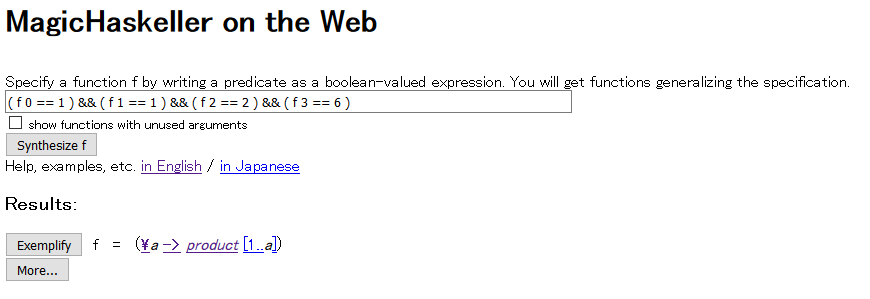
\includegraphics[width=\textwidth]{C7/magichaskeller.png}
\caption{MagicHaskeller UI}
\label{fig:magichaskeller}
\end{figure}

\subsubsection{Igor II}
Igor II \cite{Kitzelmann2006} is based on the analytical approach to IFP and is specialised towards learning recursive programs. It works by first calculating the \textit{least-general generalisation} of the examples, which extracts terms which are common between the examples and terms which are uncommon are represented as variables. If this initial hypothesis is incomplete (i.e not a correct functional program) then four refinement operators are applied to attempt to complete it:
\begin{enumerate}
\item Partition the examples into two subsets and generate a new, more specific least general generalisation for each subset. This partition is calculated using pattern matching on the variables from the lhs of the initial hypothesis.
\item If the rhs of the initial hypothesis has a function as its root element then each unbound argument of this function is treated as a subproblem, and new functions are introduced for each argument.
\item The rhs of the initial hypothesis may be replaced by a recursive call to a user-defined function, where the arguments of this call are newly introduced functions.
\item If the examples match certain properties then a higher order function may be introduced, and synthesising the arguments to this function becomes the new induction problem.
\end{enumerate}
Igor II has a number of limitations. If there are a large number of examples then performance can be impacted because of the large number of combinations when matching to a defined function. Synthesis can fail or perform incorrectly if some examples from the middle of the set are removed, meaning if we want to specify a particularly large or complex example we also have to specify all of the smaller examples, reducing performance.

\subsubsection{FlashFill}
FlashFill \cite{Gulwani2012} is an Inductive Program Synthesis system which generates string and table operations over spreadsheets columns. By defining a domain specific language that is expressive enough to efficiently describe the potential string operations, this language is used to define a data structure which represents the set of possible functions in a succinct manner. \\ \\
These functions are then learned in a two-step procedure. First, for each example, the set of all potential functions that transform the given input to the given output is generated. While this set could be very large, it is optimised by reducing the number of potential substrings of a string be quadratic, not exponential in the size of the string. After this set is generated for each example, the sets are examined to find matching cases and learn conditionals to determine between them. These solutions are then optimised, with shorter expressions being preferred in general.\\ \\
FlashFill is fairly unique in the field of program synthesis due to the fact it has been implemented as a consumer tool. Included in Microsoft Excel 2013, it allows users to quickly generalise an operation over multiple spreadsheet rows.

\begin{figure}[h!]
\centering
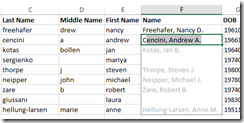
\includegraphics[width=0.4\textwidth]{C2/flash_fill.png}
\caption{FlashFill UI}
\label{fig:flashfill}
\end{figure}
\mbox{}\\
However FlashFill has been described as a ``controversial feature'' due to its simplicity. John Walkenbach, an Excel textbook author, wrote ``It's a great concept, but it can also lead to lots of bad data. (...) Be very careful. (...) [M]ost of the extracted data will be fine. But there might be exceptions that you don't notice unless you examine the results very carefully'' \cite{Bauer2016}.

%\renewcommand\bibname{{References}}
%\bibliography{References}
%\bibliographystyle{plain}

\pagebreak